
% -*- root: These.tex -*-

\subsection{Une lecture pluridisciplinaire des problématiques liées à la validation}
\label{ssec:triple_lecture}

\subsubsection{Les définitions de la validation en V\&V}
\label{sssec:def_generique_validation}

Les termes \foreignquote{english}{Validation \& Verification} ou \textit{V\&V} proviennent à l'origine de l'ingénierie des systèmes et peuvent être rattachés au concept de \enquote{qualité} tel qu'il est défini par la famille de règles ISO établies par l'organisation mondiale de normalisation.

Décomposable en plusieurs branches cette discipline à part possède une branche dédiée à l'expertise logicielle. De ce fait, il n'existe pas réellement de définition ni de théories ou méthodologies officiellement acceptables, l'acceptation des termes pouvant varier fortement selon les branches d'application.

On trouve toutefois quelques références dans des livres dédiés à la terminologie standard pour la \enquote{gestion de projet} dans un large panel de disciplines, telle que le PMBOK (\textit{A guide to the project Management Body of Knowledge}) \autocite{PMBOK2013}. Résultats d'un travail certifié par des associations ou des organismes étatiques tels que IEEE et ANSI, ce dernier propose une définition générale de ces termes pour l'ingénierie logicielle :

\foreignquote{english}{Verification and validation (V\&V) processes are used to determine whether the development products of a given activity conform to the requirements of that activity and whether the product satisfies its intended use and user needs.}

et revient ensuite plus spécifiquement sur les termes :

\begin{itemize}
\item \textbf{Validation} \foreignquote{english}{The assurance that a product, service, or system meets the needs of the customer and other identified stakeholders. It often involves acceptance and suitability with external customers. Contrast with verification.}
\item \textbf{Verification} \foreignquote{english}{The evaluation of whether or not a product, service, or system complies with a regulation, requirement, specification, or imposed condition. It is often an internal process. Contrast with validation.}
\end{itemize}

Les termes tels qu'ils sont définis sont finalement bien trop généraux pour envisager de les appliquer tels quels dans notre domaine de compétence. Dérivés de la branche de l'\textit{Operational Research (OR)}, les auteurs de la communauté restreinte des \textit{systems analysis or modelling and Simulation (M\&S) } engagent dès les années 1960-70 des efforts pour standardiser ces définitions pour la simulation.

Parmi les différents auteurs participant de ce mouvement ( Naylor, Finger, Oren, Hermann, Zeigler, Nance, Banks, Gass, Balci, Sargent, etc.), \textcite{Naylor1966} sont considérés avec West Churchman (1963) comme les tout premiers à avoir attiré et cristallisé \Anote{first_time_validation} dans de multiples publications l'attention sur cette problématique importante de la V\&V.

Formé à l'informatique dans la branche des \foreignquote{english}{management sciences} \autocite{Stricklin1985}, Naylor est un des premiers en 1967 \autocite{Naylor1967} à publier dans un article nommé \foreignquote{english}{Verification of Computer simulation models} une méthode abordant spécifiquement la question de la crédibilité des connaissances qui peuvent être apportées par un modèle de simulation. Une méthode qu'il va mettre spontanément en tension avec les débats qui agitent la communauté des philosophes à cette même période.

Malgré ses efforts et sa volonté de porter le débat loin dans la communauté interdisciplinaire (voir les premiers ouvrages collectifs sur l'usage de la simulation dans les \textit{behavior science} \autocites{Dutton1971, Guetzkow1972} ), la démarcation entre les deux termes reste encore peu claire à cette période \Anote{naylor_nance} \autocites[165]{Nance2002}[3]{Balci1986}.

Il faudra attendre le début des années 1980 pour qu'un standard émerge, grâce à des financements étatiques \autocite{Balci1986}, mais également du fait des efforts fournis par des auteurs comme Sargent et Balci \autocite{Nance2002}, qui collectent et organisent dans une typologie cohérente l'existant statistique et méthodologique, une activité qu'ils poursuivent encore aujourd'hui \autocite{Balci1998}.\Anote{balci_standard}

Pour \textcite[22]{Oberkampf2010} \foreignquote{english}{A Key milestone in the early work by the OR community was the publication of the first definitions of V\&V by the Society of Computer Simulation (SCS) in 1979 \autocite{Schlesinger1979}}. La SCS est un des instituts avec la U.S GAO (U.S General Accounting Office) à fournir des spécifications en 1979 \autocite{Balci1986}.

\begin{itemize}
\item \textbf{Model Verification} \foreignquote{english}{substantiation that a computerized model represents a conceptual model within specified limit of accuracy.}
\item \textbf{Model Validation} \foreignquote{english}{substantiation that a computerized model within its domain of applicability possesses a satisfactory range of accuracy consistent with the intended application of the model.}
\end{itemize}

\begin{figure}[h]
\begin{sidecaption}[fortoc]{Un des tout premiers schémas issus de la publication de la SCS \autocite{Oberkampf2010,Schlesinger1979}}[fig:S_VV]
  \centering
 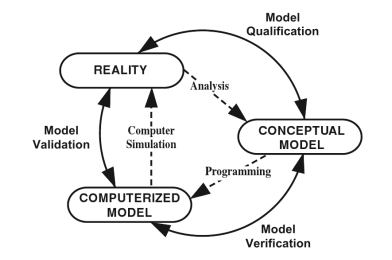
\includegraphics[width=.7\linewidth]{schelinger_schema1979.png}
  \end{sidecaption}
\end{figure}

Même si elles sont plus anciennes et de portée moins générale, ces définitions de la \textit{V\&V} semblent plus pertinentes, car évoquées plus régulièrement par les chercheurs en sciences sociales; les travaux les plus cités étant ceux de \textcite{Kleijnen1995}, ou \textcite{Sargent2010} qui placent leurs travaux dans la continuité de ces définitions. L'avancée de leurs travaux peut être suivie en feuilletant les \textit{Proceedings of the Winter Simulation Conference} où la problématique de la \textit{V\&V} est réévaluée régulièrement au regard des nouvelles connaissances. Ce schéma \ref{fig:S_VV} est devenu un classique repris et régulièrement amendé \autocite{Sargent2010}. Voici la lecture qu'en fournit \autocite{Oberkampf2010}

\foreignquote{english}{The \textbf{conceptual model} comprises all relevant information, modelling assumptions, and mathematical equations that describe the physical process or process of interest. [...] The SCS defined \textbf{qualification} as \enquote{Determination of adequacy of the conceptual model to provide an acceptable level of agreement for the domain of intended application}. The \textbf{computerized model} is an operational computer program that implements a conceptual model using computer programming. Modern terminology typically refers to the computerized model as the computer model or code.}

Ce schéma a la particularité suivante, il \foreignquote{english}{ [...] emphasizes that \textbf{verification} deals with the relationship between the conceptual model and computerized model and that \textbf{validation} deals with the relationship between the computerized model and reality. These relationships are not always recognized in other definitions of V\&V [...]}


Autrement dit, \foreignquote{english}{The OR community clearly recognized, as it still does today, that V\&V are tools for assessing the accuracy of the conceptual and computerized models.} Un avis partagé par \textcite{Kleijnen1995} \Anote{Kleijnen_def} , \textcite{Balci1998}, et \textcite{Sargent2010} \Anote{Sargent_def}.

Seulement, cette forme de relâchement sur la correspondance entre réalité et modèle, et ce positionnement plus relativiste de la validation n'a pas toujours été une évidence; les premières définitions de Naylor par exemple, sont toujours usitées et continuent si on en croit des auteurs comme \textcite{Kleindorfer1998} à semer le trouble dans certaines disciplines.

Mais en excluant ainsi de son analyse la partie subjective et philosophique de la \enquote{Validation} \Anote{VV_philout} pour se concentrer sur la seule partie opérationnelle, ces méthodologies restent pour le modélisateur une coquille vide décevante, qui demande encore à être incarnée thématiquement. Autrement dit, ces méthodes si elles prennent bien en compte la dimension dynamique et incrémentale nécessaire à la construction d'un modèle de simulation qui tendrait vers une réalité en accord avec la question posée, l'organisation des connaissances nécessaires pour guider ce processus reste à la lecture de ces typologies une opération quelque peu énigmatique pour les modélisateurs géographes. On retombe sur une des critiques soulevées précédemment dans la section \ref{sec:critiques_simulation} sur l'absence constatée dans les publications de méthodologie standard pour la validation qui prendrait en compte les problématiques spécifiques d'une discipline.

Une position compréhensible de ces auteurs oeuvrant pour la standardisation, alors même que ces termes restent d'usages assez variables selon les disciplines. Une des conséquences visibles tient dans ces incompréhensions et ces débats terminologiques sans fin \autocites{David2009, Augusiak2014} que l'on observe parfois en marge des discussions interdisciplinaires. Cette gamme d'acceptions différentes tient souvent au transfert hasardeux des terminologies entre l'ingénierie des M\&S, la philosophie des sciences, et la thématique d'un chercheur en sciences sociales qui se retrouve en position intermédiaire de ces deux derniers. Un exercice d'équilibriste périlleux, car comme le fait remarquer \textcite{Kleijnen1995} en citant astucieusement une note de bas de page de \textcite{Barlas1990}, en philosophie il est tout à fait possible de voir la signification des deux termes inversée\Anote{philo_verification} !

\subsubsection{La philosophie des sciences}
\label{sssec:philo_sciences}

Il ne s'agit pas de se lancer ici dans un exposé historique des courants et débats s'étant succédés dans cette discipline, mais d'amener de façon illustrative et avec quelques références récentes l'émergence ces 20 dernières années d'une \enquote{épistémologie de la simulation} reprenant (en parasitant parfois le débat comme on l'a cité au-dessus) de son point de vue certains débats évoqués chez les praticiens de la simulation; la question de validation traitée dans le chapitre 1 étant un sujet de longue date chez les praticiens de la simulation, mais aussi chez les premiers acteurs fondateurs de la V\&V.

\hl{redite : L'objectif n'est donc pas tant de développer une argumentation critique exposant l'ensemble de ces points de vue, car ce n'est pas l'objet de cette thèse, que de tenter de s'insérer (et non de s'enfermer) dans ces réflexions en spécifiant en quoi celles-ci diffèrent, négligent ou font peu écho à nos pratiques et réflexion historique en sciences sociales.}

Le premier obstacle avec laquelle les acteurs supportant cette nouvelle épistémologie doivent cohabiter est évidemment la contre-argumentation questionnant cette même nécessité d'opérer une nouvelle sous-division épistémologique. Car existe-t-il réellement des spécificités à la connaissance dérivée de l'étude de l'objet simulation, et si oui quelles sont-elles réellement ? Autrement dit, existe-t-il une différence fondamentale entre les questionnements déjà posés dans le cadre d'une épistémologie des modèles et ceux évoqués dans le cadre d'une épistémologie de la simulation ?

\Anotecontent{frilosite_philoScience}{\foreignquote{english}{As computer simulation methods have made their way into novel disciplines, the issue of their trustworthiness for generating new knowledge has often loomed large, especially when they have competed for attention with experiments or analytically tractable modeling methods. The relevant question is always whether or nhorizonot the results of a particular computer simulation are accurate enough for their intended purpose.[...] Given our long-standing preoccupation with issues of confirmation, it might seem obvious that philosophers of science would have the resources to easily approach these questions.} \autocite{Winsberg2013}}

Parmi les auteurs ouvertement favorables à la création d'une nouvelle épistémologie, on citera entre autre les efforts de \autocites{Winsberg2001, Winsberg2009, Winsberg2013} qui pousse dans chacune de ses publications les \enquote{philosophes des sciences} à sortir de la seule étude de la \enquote{théorie de la confirmation} pour aller vers un terrain un peu plus aventureux \Anote{frilosite_philoScience}, celui de l'étude de la crédibilité des explications et des hypothèses dans leur dépendance au contexte.

Il propose de résumer l'originalité d'une telle épistémologie en évoquant l'inférence spécifique que produit l'étude simultanée de trois points sur la simulation. \foreignquote{english}{ \textcite{Winsberg2001} argued that, unlike the epistemological issues that take center stage in traditional confirmation theory, an adequate EOCS must meet three conditions.
downward, motley, and autonomous.[...] These three features were meant to be offered as conditions of adequacy; for which any adequate epistemology of simulation must account. Against the background of the growing use of simulation in the sciences, an adequate epistemology for the philosophy of science needs to explain the fact that simulation results and computational models are often taken to be reliable despite these three features. Winsberg (2001) argues that simulation requires a new epistemology precisely because traditional stories in philosophy of science about how knowledge claims get credentialed cannot explain them.}

Cette typologie a soulevé un certain nombre de critiques chez les philosophes des sciences, dont la plus longue et la plus argumentée est surement celle de \textcite{Frigg2009} dont on trouve le résumé des points saillants dans les publications de \textcites{Winsberg2009, Winsberg2013} mais également de bien d'autres auteurs qui se réfèrent à ce débat pour se positionner \textcites{Yanoff2010, Eckhart2010}.

Le deuxième point de débat intéressant réside dans le qualificatif souvent donné à la simulation de \enquote{laboratoire virtuel pour l'expérimentation}. Si les philosophes des sciences ne peuvent que s'incliner face au constat d'une telle banalisation du terme, dont nous avons donné nous-mêmes un aperçu de son ancienneté d'usage dans les sciences sociales dans le chapitre 1; il existe quand même chez les philosophes la volonté de mettre à l'épreuve les fondements et les conséquences pour la connaissance extraite d'une telle analogie.

\Anotecontent{HackingCartwright}{\enquote{Nos deux livres ont plus d'un point commun. L'un et l'autre accordent peu d'importance à la vérité des théories et avouent un faible pour certaines entités théoriques. Cartwright soutient que seules les lois phénoménologiques de la physique parviennent à la vérité tandis que, dans la partie B de ce livre, je fais remarquer que la science expérimentale est plus indépendante de la théorie que ce que l'on veut bien généralement admettre. Nous ne partons pas des mêmes postulats anti-théoriques car elle considère les modèles et les approximations alors que c'est surtout l'expérience qui m'intéresse, mais nos conceptions convergent.}\autocite{Hacking1989}}

\Anotecontent{Phan_Varenne_theorie}{\foreignquote{english}{Consequently, in the first neo-positivist epistemology, models were viewed not as autonomous objects, but as theoretically driven derivative instruments. Following the modelistic turn in mathematical logic, the semantic epistemological conception of scientific models persisted to emphasize on theory.} \autocite{Phan2010}}

Un débat d'autant plus actif qu'on assiste depuis ces 20 dernières années à un véritable renouveau des questionnements dans le cadre d'une \enquote{épistémologie de l'expérimentation} jusqu'alors relativement peu considérée par la majorité des philosophes des sciences \Anote{Phan_Varenne_theorie}. \textcites{Phan2008, Phan2010} citent ainsi les contributions importantes d'auteurs comme Fischer(1996), Galison (1987, 1997), Franklin (1986, 1996), Morrisson(1993, 1999), mais également les efforts de Hacking (1983) et Cartwright.

\Anotecontent{def_cartwright}{\enquote{Disons qu'il y a des théories, des modèles et des phénomènes. Il serait normal de penser que les modèles sont doublement des modèles. Ils sont modèles pour les phénomènes et modèles pour la théorie. [...] Le réalisme scientifique est ici tout particulièrement concerné. Cartwright est pour l'essentiel anti-réaliste à propos des théories. Pour cela, elle s'appuie en partie sur les modèles. Elle fait remarquer que non seulement les modèles ne peuvent être déduits de la théorie qui les englobe, mais plus encore que les physiciens utilisent à leur gré divers modèles qui, sans pourtant se recouper, cohabitent tous au sein de la même théorie. Et cependant,ces modèles sont les seules représentations formelles disponibles des lois phénoménologiques que nous tenons pour vraies. Elle affirme que seules ces lois phénoménologiques nous permettent d'avancer. Toutes les modélisations de ces lois ne peuvent être vraies ensemble puisqu'elles ne sont pas compatibles. Et rien ne permet de penser qu'un modèle est supérieur à un autre. Aucun n'est vraiment justifié par la théorie qui le porte. Plus encore, les modèles ont tendance à résister aux changements de théorie, c'est-à-dire que le modèle est conservé même si la théorie s'avère inadéquate. Il y a plus de vérité locale dans les modèles incompatibles que dans les théories, pourtant plus sophistiquées.[...] L'idéal de la science n'est pas l'unité mais dans une abondance et diversité de plus en plus grandes.} \autocite[350]{Hacking1989}}

\Anotecontent{def_hacking}{\enquote{Le \textit{réaliste à propos des entités} affirme que bon nombre d'entités théoriques existent vraiment. L'anti-réaliste s'oppose à ces entités qui ne sont pour lui que fictions, constructions logiques ou éléments d'un processus intellectuel d'appréhension du monde. Un anti-réaliste moins dogmatique dirait que nous n'avons pas, et ne pouvons avoir, de raison de supposer que ces entités ne sont pas des fictions. Peut-être existent-elles, mais le présupposer n'est pas nécessaire à notre compréhension du monde.

Le \textit{réaliste à propos des théories} dit que les théories
sont soit vraies, soit fausses et ce indépendamment de ce que nous percevons : la science, elle au moins, vise à obtenir la vérité et la vérité est le monde tel qu'il est. L'anti-réaliste dit des théories qu'elles sont au mieux prouvées, adéquates, opératoires, acceptables - quoi que incroyables, entre autres qualificatifs possibles.} \autocite[59]{Hacking1989}}

On retiendra principalement pour notre argumentaire cette propriété d'indépendance retrouvée de l'expérimentation par rapport à la théorie \Anote{def_cartwright}, dont on peut trouver un très bon manifeste dans les écrits de \textcite{Hacking1989} et Cartwright \Anote{def_hacking}, ces derniers se positionnant comme des antiréalistes des théories, tout en étant des réalistes des entités théoriques. Un point de vue très bien résumé à la fois dans \textcite{Hacking1989} et \textit{Théorie, Réalité, Modèle} de \textcite[226-231]{Varenne2012}

Sur la notion de modèle dans sa relation à l'expérimentation, il semblerait qu'un consensus se dégage chez les philosophes \autocites{Morgan2009, Varenne2013} autour du modèle perçu comme un \enquote{médiateur autonome} articulant théorie, pratiques et données dans un contexte spécifique d'une question et d'un cadre technico-social. \autocite[2]{Phan2010}

Il y a probablement un point intéressant à développer entre cet argument du modèle autonome, et les récents travaux en sciences sociales pour qualifier au travers d'une grille de lecture \autocites{Banos2013a, Sanders2013} le positionnement \autocites{Banos2013, Schmitt2013} et le déplacement des modèles de simulation au travers d'une part de leur construction \autocite{Cottineau2014b}, mais également de leur réutilisation \autocite{Schmitt2014}. Une autre façon de démontrer en quoi cette capacité à cumuler de façon floue différentes fonctions épistémiques données dans la spécification minimale de Varenne pour la simulation \autocite{Varenne2013} est intéressante dès lors qu'il s'agit de tracer la trajectoire disciplino-temporelle de certains modèles : daisyWorld \autocite{Dutreuil2013}, Schelling \autocite {Bulle2005}, SugarScape, etc.)

\Anotecontent{winsberg_exper_simu_link}{Another unique feature of the epistemology of simulation is the ease with which it can draw inspiration from the epistemology of experiment.}

Les acteurs prônant comme Winsberg une épistémologie de la simulation n'hésitent alors pas à débattre pour ce qui est des différents parallèles que l'on peut tracer avec les réflexions de cette communauté. \Anote{winsberg_exper_simu_link}.

Pour ne pas se perdre dans les différents points de vue sur le sujet et bénéficier d'une vue plus large incluant les réflexions des praticiens, on pourra se référer au travail opéré par \textcite{Varenne2001} dans son article \textit{What does a computer simulation prove?}, qui propose une lecture du débat au travers d'une typologie soulevant trois grandes thèses : I - La simulation est-elle un outil commes les autres \textit{A simulation is only a tool} ? II - ou bien l'équivalent fusionnel d'une expérimentation classique (\textit{A simulation is an experiment}) ? III - ou se positionne-t-elle comme médiateur entre la théorie et expérimentation ? (\textit{A computer simulation is an intermediate between theory and experiment})?

%L'expérimentation mène sa vie propre et entretient diverses relations avec la spéculation, le calcul, la construction de modèles, l'invention et la technologie. Mais alors que le calculateur, le spéculateur et le constructeur e modèles peuvent être anti-réalistes, l'expérimentateur, lui, doit être réaliste. p18

On trouve donc un grand nombre de travaux, toutes disciplines confondues (les philosophes des sciences ne sont pas les seuls à se poser ce type de question, comme nous verrons par la suite), qui tentent d'établir par le biais de différentes grilles de lecture l'appartenance de ce \enquote{nouveau?} mode d'expérimentation à une des catégories de cette grille. \textit{Pourquoi ? Au delà du jeu d'esprit, quel est l'enjeu motivant une telle comparaison ?}

\Anotecontent{moto_hacking}{Une remarque qui renvoie d'ailleurs explicitement à sa lecture du moto d'Hacking \foreignquote{english}{experiments have a life of their own} et à la notion d'autonomie (\textit{autonomous}) de sa synthèse précédemment, qui marque le fait que dans certains cas (impossibilité d'observation, manque de données), la simulation doit faire la preuve des connaissances (\textit{background knowledge}) apportées sur appel de ses propres ressources.}

\Anotecontent{experimental_warranting_belief}{\foreignquote{english}{The central idea of this thread is that experiments are the canonical entities that play a central role in warranting our belief in scientific hypotheses, and that therefore the degree to which we ought to think that simulations can also play a role in warranting such beliefs depends on the extent to which they can be identified as a kind of experiment} \autocite{Winsberg2009}}

Partant du fait que l'expérimentation joue un grand rôle dans l'établissement d'une crédibilité pour les hypothèses avancées, il s'agit de mesurer à quel point la simulation serait susceptible d'apporter les mêmes garanties dès lors qu'on accepte de la voir comme une sorte d'expérimentation.\Anote{experimental_warranting_belief}

On s'appuiera dans la suite de cette argumentation sur la lecture de Winsberg, un philosophe des sciences que l'on estime plutôt partisan de la thèse III dans la classification ci-dessus. Ce dernier s'appuie largement sur les travaux d'Hacking, mais aussi Galison pour construire sa réflexion, par exemple en arguant\foreignquote{english}{ [...] that some of the techniques that simulationists use to construct their models get credentialed in much the same way that Hacking says that instruments and experimental procedures and methods do; the credentials develop over an extended period of time and become deeply tradition-bound.} \autocites{Winsberg2003, Winsberg2013} \Anote{moto_hacking}

Winsberg résume ce débat en deux thèses opposées : \foreignquote{english}{Identity Thesis} qui consiste à dire que la simulation est littéralement une expérimentation, et \foreignquote{english}{Epistemology Identity Thesis} qui consiste à penser qu'il existe une dépendance entre les garanties de crédibilité qui pourront être accordées par les résultats de la simulation et leur capacité à être plus ou moins définie en tant qu'expérience. Si la première thèse semble assez bien correspondre au point I de la classification de Varenne, la deuxième semble être une sous-variation du point I.

La plupart des auteurs cités par la suite dans ce débat sont des philosophes des sciences spécialisés en économie (Guala , Morgan, Maki, Simon ) qui rejettent comme Winsberg (plus spécialisé en physique) assez naturellement ces deux thèses \autocite{Winsberg2009}, mais avec des arguments assez différents, qu'il convient d'évoquer pour bien comprendre la complexité de ce débat, assez théorique.

\Anotecontent{maki_phan}{\foreignquote{english}{For Mäki, abstractions in models are similar to abstractions in experiments as they both can be interpreted as a kind of isolation [...] This analogy between models and experiments is called \enquote{isolative analogy} by Guala (2008). From Mäki’s standpoint, a model can be said to be experimented in its explanatory dimension: the finality of such a model is to explore the explanatory power of some causal mechanism taken in isolation.} \autocite{Phan2008}}

Parmi les différents point de vue existants, on citera par exemple le sous-débat de l'\foreignquote{english}{isolative analogy} relaté ici au travers des publications de \textcite{Phan2008, Phan2010} appelant les points de vue de Morgan et Guala contre Maki (2005). Ce dernier voit dans la similitude entre isolement théorique du modèle comme expérience de pensée et isolement expérimental \Anote{maki_phan} la possibilité de rejoindre une des deux thèses évoquées par Winsberg, établissant d'une façon ou d'une autre que \textit{les modèles sont des expériences, et les expériences des modèles}. Mais ce type d'argument, et on le suppose tous ceux qui se rapportent à l'évocation d'analogies pour justifier d'une équivalence de puissance épistémique se heurteraient, comme on va le voir, à une différence fondamentale.

\Anotecontent{guala_phan_winsberg}{Winsberg résume le point de vue de Guala(2002) ainsi \foreignquote{english}{Guala argues that simulation differ fundamentally from experiments in that the object of manipulation in an experiment bears a material similarity to the target of interest, but in a simulation, the similarity between object and target are merely formal.}, mais on peut trouver une version réactualisé en 2008 dans l'article de \textcite[4.2]{Phan2010} \foreignquote{english}{In a simulation, one reproduces the behavior of a certain entity or system by means of a mechanism and/or material that is radically different in kind from that of a simulated entity (...) In this sense, \enquote{models simulate} whereas \enquote{ experimental systems} do not. Theoretical models are conceptual entities, whereas experiments are made of the same \enquote{stuff} as the target entity they are exploring and aiming at understanding}\autocite[14]{Guala2008}}

\textcite{Phan2010} et \textcite{Winsberg2013} citent le point de vue de Guala (2002, 2008), partagé par Morgan(2002, 2005) et se référent aux travaux de Simon (1969). Ceux-ci s'appuient sur une différence de relation qui existe entre système à étudier et système cible dans chacun des deux cas. En effet, dans le cas des expériences, la comparaison s'appuie avant tout sur une similarité matérielle, alors que dans le cas de la simulation la comparaison est limitée à une comparaison formelle entre les objets.\Anote{guala_phan_winsberg}

\Anotecontent{Winsberg_critique_morvan}{\foreignquote{english}{Interestingly, while Morgan accepts this argument against the identity thesis, she seems to hold to a version of the epistemological dependency thesis. She argues, in other words, that the difference between experiments and simulations identified by Guala implies that simulations are epistemologically inferior to real experiments - that they have intrinsically less power to warrant belief in hypotheses about the real world.} \autocite[841]{Winsberg2013}}

Morgan(2002, 2005) accepte le point de vue Guala et Simon, mais s'en sert pour réduire indirectement le pouvoir épistémique de la simulation. Un argument bien résumé par \textcite{Phan2008} \enquote{Pour Morgan (2005) les modèles et expériences partagent des fonctions de médiateurs et peuvent fonctionner \textit{sur un mode expérimental}, mais les expériences \textit{réelles} offrent un \textit{pouvoir épistémique} d'investigation de la réalité empirique plus fort.} Ce qui fait dire à Winsberg que Morgan serait indirectement plutôt partisan de sa deuxième thèse.\Anote{Winsberg_critique_morvan}
\Anotecontent{winsberg_mereformal}{\hl{A compléter avec ce que dit Winsberg2013}}

Pour \textcite{Winsberg2009} le flou des arguments avancés par Morgan et Guala  (\textit{material similarity}, \textit{mere formal similarity}) ne permet pas d'exclure complétement et définitivement la première thèse.\Anote{winsberg_mereformal} Celui-ci se range malgré tout du côté de Guala, et préfère là aussi rejetter cette thèse, mais à la faveur de sa propre argumentation; ce qui lui permet de rejetter à la fois l'argument de Morgan pointant l'infériorité épistémique de la simulation, et la deuxième thèse. Il argue que les simulations et l'expérience diffère principalement par la nature du \textit{background knownledge}, c'est-à-dire les protocoles et les connaissances mobilisés.

Des modélisateurs et épistémologues en sciences sociales beaucoup plus proches de nos pratiques comme Phan et Varenne trouvent un argument convaincant dans ce dernier point, car \foreignquote{english}{Aujourd'hui, comme le souligne Winsberg, la crédibilité des modèles de simulation repose largement sur la \textit{confiance} que nous pouvons avoir dans les compétences des modélisateurs, informaticiens, expérimentateurs et observateurs, ainsi que dans les composants ou plateformes qui supportent les expériences de simulation.} \autocite{Phan2008}

\Anotecontent{gilbert_critique}{\foreignquote{english}{\enquote{[t]he major difference is that while in an experiment, one is controlling the actual object of interest (for example, in a chemistry experiment, the chemicals under investigation), in a simulation one is experimenting with a model rather than the phenomenon itself.} \autocite[14]{Gilbert2005}. But this doesn't seem right. [...] It is false that real experiments always manipulate exactly their targets of interest. In fact, in both real experiments and simulations, there is a complex relationship between what is manipulated in the investigation on the one hand, and the real-world systems that are the targets of the investigation on the other. In cases of both experiment and simulation, therefore, it takes an argument of some substance to establish the ‘external validity’ of the investigation – to establish that what is learned about the system being manipulated is applicable to the system of interest. Mendel, for example, manipulated pea plants, but he was interested in learning about the phenomenon of heritability generally \autocite{Winsberg2013}}}

\Anotecontent{guala_morgan_reality_experiments}{\foreignquote{english}{The identity thesis itself has drawn criticism from Guala (2002) and Morgan(2002). Guala begins by dismissing what he takes to be a poor argument against it. The poor argument goes something like this : simulations are not at all like real experiments because real experiments manipulate the real-world systems that are the very target of the investigation, while simulation merely manipulate \enquote{models} of the target system. What both Guala and Morgan correclty point out is that it is, quite generally speaking, false.}}

Autre sous-débat évoqué par \textcite{Winsberg2013}, on suppose en partie en réponse à son article précédent et très similaire \autocite{Winsberg2009}, la critique de l'\textit{identity thesis} comme évoqué par Gilbert et Troitzsch (1999), dont il pense \Anote{gilbert_critique}, en accord avec Guala (2002) \autocite{Winsberg2009} mais également Morgan et Parker \autocite{Winsberg2013} qu'elle est un argument trop faible pour rejeter l'\textit{identity thesis}.\Anote{guala_morgan_reality_experiments}

Si les arguments de Winsberg semblent convaincants, \textcites{Peschard2010b, Peschard2013} tente dans une analyse critique d'en montrer les biais, et apporte dans son article des objections tout à fait crédibles issues de son domaine d'expertise. Pour ne citer qu'un de ces arguments, s'il existe bien un intermédiaire de mesure issue d'un modèle, comme l'indique Winsberg, il existe également un sous système en prise directe avec la réalité physique de ce monde. En conclusion, elle estime que s'il y a bien une certaine forme de similarité entre cibles épistémiques de la simulation et de l'expérience, ces activités ne peuvent pas être épistémiquement équivalentes, ce qui n'empêche en rien selon elle la coopération fructeuse des deux approches. \hl{Ajouter une footnote avec explication}

\textcite{Winsberg2013} résume le point de vue de \autocite{Peschard2010} ainsi, \textit{Thus, simulation is distinct from experiment, according to her, in that its epistemic target (as opposed to merely its epistemic motivation) is distinct from the object being manipulated.} Autrement dit, même si la motivation menant à l'expérience est bien éloignée (la motivation), l'objet manipulé dans une expérience est bien celui du monde physique, alors que dans le cas de la simulation c'est l'ordinateur. Or autant la motivation peut apprendre de l'objet manipulé dans le monde physique, autant il n'est pas ici dans notre intérêt d'apprendre sur l'ordinateur en tant qu'objet. Dans ce cas là on pointe une différence, mais on peut également appeler selon \textcite{Winsberg2013} et Morrisson (2009) l'argument inverse pointant au contraire une similarité. L'objet expérimenté étant le plus souvent choisi en tenant compte justement de sa capacité de \textit{surrogate} rapport à la question que l'on se pose effectivement, un point commun entre la construction de simulation et d'expérimentation.

Winsberg conclut en ajoutant que l'expérimentation, contrairement à ce que l'on pourrait penser, n'est pas forcément et immédiatement plus crédible si on ne lui ajoute pas un bagage de connaissances : \textit{Experiments are not automatically more reliable than simulations, despite their differences. [...] It would seem that there are identifiable differences between ordinary experiments and simulations, but there is nothing about these differences that makes one or the other intrinsically more epistemically powerful.}  \autocites{Winsberg2009, Winsberg2013}

\textcite{Varenne2001} avance alors un autre argument intéressant : \foreignquote{english}{Indeed, when you read (Von Neumann 1951), you see that analog models are inferior to digital models because of the accuracy control limitations in the first ones. Following this argument, if you consider a prototype, or a real experiment in natural sciences, is it anything else than an analog model of itself? The test on the prototype is a real experiment. But is it something different and better than the handling of an analog model? So the possibilities to make sophisticated and accurate measures on this model - i.e. to make sophisticated real experiment - rapidly are decreasing, while your knowledge is increasing. These considerations are troublesome because it sounds as if nature was not a good model of itself and had to be replaced and simulated to be properly questioned and tested! It looks as if it was not possible any more to end a paper on simulation by reassuringly using the traditional word: \enquote{Simulation will never replace real experiments”.} }

Ces derniers paragraphes montrent que le débat est loin d'être fixé, et il semblerait là encore que ce soit la définition du contexte d'application qui détermine le mieux la capacité explicative de la simulation, car comme le dit Winsberg \enquote{l'impossibilité d'expérimenter} existe dans bien des disciplines, comme les sciences sociales, mais également la biologie ou la physique, où les tentatives de reconstitution simulées d'univers ou d'étoiles dans des super calculateurs de plus en plus puissants montrent qu'il existe un interêt explicatif à cette pratique. On pensera notamment aux projets d'expérimentation récents extrêmement complexes et coûteux en physique (laser megajoule de bordeaux, projet ITER pour la fusion).

Et c'est sur ce point que l'argumentation de la plupart des philosophes des sciences est tout à la fois aussi intéressante que problématique. Pour continuer sur Winsberg, celui-ci traite de ces problématiques en se positionnant uniquement du point de vue des sciences physiques. Un fait dont il reconnaît prudemment les conséquences que peuvent avoir l'inclusion d'un contexte différent sur sa synthèse : \foreignquote{english}{Parker (forthcoming) has made the point that the usefulness of these conditions is somewhat compromised by the fact that it is overly focused on simulation in the physical sciences, and other disciplines where simulation is theory-driven and equation-based. This seems correct. In the social and behavioral sciences, and other disciplines where agent-based simulation (see 2.2) are more the norm, and where models are built in the absence of established and quantitative theories, EOCS probably ought to be characterized in other terms.

For instance, some social scientists who use agent-based simulation pursue a methodology in which social phenomena (for example an observed pattern like segregation) are explained, or accounted for, by generating similar looking phenomena in their simulations (Epstein and Axtell 1996; Epstein 1999). But this raises its own sorts of  epistemological questions. What exactly has been accomplished, what kind of knowledge has been acquired, when an observed social phenomenon is more or less reproduced by an agent-based simulation? Does this count as an explanation of the phenomenon? A possible explanation?
(see e.g., Grüne-Yanoff 2007).

It is also fair to say, as Parker does (forthcoming), that the conditions outlined above pay insufficient attention to the various and differing purposes for which simulations are used (as discussed in 2.4). [...] Indeed, it is also fair to say that much more work could be done in classifying the kinds of purposes to which computer simulations are put and the constraints those purposes place on the structure of their epistemology.}

Des philosophes des sciences ont donc saisi cette opportunité de critiquer l'approche de Winsberg pour soulever dans des tentatives de typologies parfois intéressantes \autocite{Eckhart2010} les points de divergences que soulève l'utilisation d'une philosophie des sciences naturelles inadaptée à la simulation en sciences sociales. Malheureusement, au cours de ces mêmes lectures, on constate que cette critique se retourne vers les modélisateurs et praticiens des sciences sociales, et mène cette fois-ci dans une analyse incomplète du contexte historique au mieux à des interprétations erronées (voir le débat animé entre \autocite{Yanoff2008}  \autocites{Elsenbroich2012, Chattoe2011}), et au pire à des approximations et conseils de mise en oeuvre totalement déplacés \autocite{Eckhart2010} vis-à-vis de disciplines qui disposent comme on l'a vu d'une véritable histoire autour de l'usage des méthodes computationelles.

Car bien que la recherche des points communs et des différences entre réalité de l'expérimentation physique et virtuelle apparaisse comme un débat intéressant, il faut bien avouer que celui-ci ne peut que difficilement s'adapter à la quasi absence d'expérimentation au sens classique dans les sciences sociales. Ainsi, même si la simulation partage certaines des propriétés de l'expérimentation classique, il y a quand même quelque chose de paradoxal à vouloir absolument analyser le rapport de la simulation à l'expérimentation alors même que c'est cette absence qui justement motive son utilisation dans notre discipline, hormis peut-être pour mettre plus en avant cette incapacité à formuler un unique cadre fédérateur par un tel débat. Comme le dit très justement \textcite{Phan2008} {[...] les sciences économiques et sociales sont plus volontiers concernées par l’opposition entre \enquote{le modèle et l’enquête}  (Gérard-Varet et Passeron, 1995) que par celle entre \enquote{l’expérience et le modèle} (Legay, 1997)}

La notion de modèle vue comme médiateur autonome entre théorie et modèle doit elle aussi être repensée pour les sciences humaines et la géographie; car les théories si elles peuvent exceptionnellement servir à dériver des modèles, celles-ci ne peuvent qu'être difficilement rapportées à leur équivalent en science physique \autocite{Pumain1997}.

D'un côté les sciences physiques semblent encore viser l'établissement d'un cadre fédérateur alors qu'il semble que les théories et les modèles en sciences sociales - hormis peut-être le cas particulier de l'économie - soit au contraire pourvoyeur de richesse dans leur capacité à apporter un nouvel éclairage sur un phénomène observé. \hl{a préciser peut etre}

A cela il faut ajouter que le modèle en géographie opère dans un cadre épistémique particulier qui n'est pas forcément celui de toutes les sciences humaines. Ainsi, bien que les notions et le rapport entre les notions d'observation du \textit{singulier} et du \textit{général} soient théoriquement à la portée de toutes disciplines \autocite{Dastes1992}, il semblerait que la géographie trouve un intérêt particulier pour la constitution de sa démarche explicative à articuler des éléments de connaissance pris dans les grandes familles explicatives historiques, écologiques, et spatiales; justifiant ainsi de niveaux d'explication plus ou moins en interaction mobilisant chacun des déterminants de nature différente. Avec la possibilité d'intégrer à tout moment dans l'explication les résidus qui tiennent d'un dialogue entre mécanismes généraux et singularité historique, écologique ou spatiale. Car quelque soit le registre explicatif choisi il reste dans les deux cas \textit{ [...] une part d'explication relevant de ce que l'on peut qualifier de singularités locales, non prédictibles à partir de mécanismes généraux, mais nécessitant d'appréhender l'histoire spécifique du lieu}. La conséquence étant une diversité de modèles support de l'explanan (l’explication que l’on propose du phénomène auquel on s’intéresse) dont l'évolution sur la forme et le fond n'a eu de cesse d'éclairer l'explanandum sous un jour différent. \autocite{Dastes1992, Sanders2000, Sanders2013} \hl{Mais il y a aussi le multi-échelles.}

\hl{A mieux introduire ici} En 1986, lors d'un débat sur les apports de l'AI en géographie, avec les apports de la branche discrète de la simulation, Couclelis montre que les considérations philosophiques abordées jusqu'ici sont en réalité très vite abordées par les géographes \foreignquote{english}{A further insight to emerge from discrete model theory, which has some interesting philosophical implications, deserves a few comments. The widespread belief that proposing a model corresponds to the assertion that the real phenomena must have some similar structure is contradicted by the sharp distinction between structure and behavior drawn in discrete model theory. Although structure governs behavior, the converse is not true, so that obtaining a model that reproduces some behavior well does not entitle one to make any inferences about the \enquote{real} structure of the phenomenon represented. In fact, it is doubtful whether we may talk about the structure of real phenomena in other than a metaphorical sense. A real system may be no more than the universe of potentially acquirable data.} \autocite{Couclelis1986}

L'éclairage sur la méthodologie sous-jacente à la construction des modèles, pourtant un élément au coeur du raisonnement dans la discipline géographique depuis la révolution quantitative, a encore moins de chance d'être évoqué dans ces publications philosophiques, au détriment d'une réflexion statique plus axée sur la nature de l'objet simulation, et de sa relation au monde.

Or l'évolution des réflexions touchant l'activité de modélisation se construit il me semble à une échelle de réflexion tout à fait différente, celle contextualisée de pratiques guidées par une activité de résolution de questions spécifiquew à l'analyse spatiale, dont la mise en oeuvre s'appuie sur une chaîne de traitements flexibles utilisant à bon escient et de façon cumulative l'arrivée historique de nouveaux outils et avec eux leur capacité à renouveler les questionnements : les statistiques, les modèles, les modèles de simulation.

\Anotecontent{Ce qui n'est pas sans nous rappeller les difficultés évoquées dans le chapitre 1 sur l'inadéquation et le danger que représentent les modes de transmissions actuels.}

\Anotecontent{remarque_Varenne_2001}{\foreignquote{english}{The second thesis of this article is that none of the three categories of arguments could be applied to contemporary sciences in general, whatever their objects, their methods and the moment of their history we consider. None of these three categories could be considered as the only true one. We cannot have a general point of view on the value of computer simulations, because of the different implications and meanings of mathematics in the different fields of science, and because of the various philosophies of nature at stake. This fact remains true for a given field throughout its own history, because the role of mathematics and the definition of the studied object evolve: You cannot find a unique and stable value that would be given to its simulation uses once for all. Again and hopefully, this thesis illustrates the fact that it does not belong to the historian to decide on the value of computer simulation in a given field but to the scientists themselves. These preliminary reflections prove the importance to investigate the intellectual history of contemporary sciences and not only their sociological construction nor their philosophical general insights.}\autocite{Varenne2001}}

Ces rapides remarques nous éclairent sur la latence qui existe entre la réflexion récente d'épistémologues comme Winsberg, Grüne-Yanoff et la réalité théorique et pratique en géographie. \textcite{Varenne2001} avait déjà bien cerné dans la synthèse faite en 2001 qu'il n'y avait pas dans sa classification une position meilleure ou plus convaincante qu'une autre, la réponse se trouvant comme pour la notion de modèle avant tout dans l'étude du contexte, et donc de l'histoire des disciplines face à cet objet simulation. \Anote{remarque_Varenne_2001} Cela ne veut pas dire que les débats évoqués précédemment en sont automatiquement invalidés, seulement qu'il faut être probablement plus regardant vis-à-vis des remarques générales et des conclusions beaucoup trop hâtivess qui peuvent parfois en découler.

Les travaux croisés de praticiens (Pumain, Sanders, Banos), d'épistémologues ou historiens des sciences propres à la géographie (Orain, Besse, Robic, Cuyala) ou s'en approchant (Varenne, Phan) permettent d'une part d'apposer un premier filtre sur ces réflexions génériques pour s'y référer prudemment, et d'autre part d'innover en questionnant nos démarches dans ce qu'elles ont d'originale, cette fois-ci appuyées sur une lecture des pratiques certes pas toujours parfaites mais pouvant au moins être qualifiées de \textit{bottom-up}.

%\hl{Un travail conséquent à la croisée de différentes approches, les travaux d'historiens et épistémologues des sciences somme Orain, Besse, Cuyala, et la lecture plus spécifique de l'évolution des méthodes numériques puis computationelles et de leur apports d'un point de vue pratique et théorique dont on trouve source à la fois dans les nombreux travaux des praticiens, mais également dans des travaux de plus long cours comme celui qu'est en train de réaliser Varenne dans son HDR.  == REDITE}

%\hl{ont su voir rapidement l'intérét de développer plus en avant les spécificités attachés à la simulation en science sociale, déjà riche de réflexion sur les apports successifs et cumulatifs de techniques de simulations \autocites{Banos2013, Varenne2008}, en s'intégrant au débat d'une communauté inter-disciplinaire structuré autour de la modélisation agent, qui émerge dans les sciences sociales au début des années 1990. Ce débat par contre ne fait semble-t-il que commencer dans le courant plus \textit{mainstream} des philosophe des sciences.}

%tel que celle des géographes pratiquant la simulation depuis les années 1950, tels que celle qui a émergé autour de la modélisation agent dans les années 1990.

%Ainsi comme on a pu le voir dans le chapitre 1, le terme laboratoire virtuel pour l'expérimentation apparait très tot dans les sciences sociales, et des auteurs ont pour l'époque déjà donnés de très bonne raisons pour l'emploi de ce terme; les aspects dynamiques de la simulation en faisait partie.

\subsubsection{La Validation vue par une communauté de modélisateurs}
\label{sssec:validation_modelisateurs}

Depuis le début des années 1990 et la diffusion progressive du méta-formalisme Agent \autocite{Treuil2008} dans les sciences humaines et sociales, les modélisateurs géographes peuvent, en plus des pratiques internes à la géographie, se tourner vers les discussions opérées dans une communauté d'acteurs internationaux et inter-disciplinaires. On trouvera à ce sujet une tentative d'exploration des fondements historiques de ce mouvement dans l'annexe \ref{double_foyer_sma}. Sorti des ouvrages fondateurs, et des ouvrages plus disciplinaires, c'est principalement autour du \textit{Journal of Artificial Societies and Social Simulation} (JASSS) fondé en 1998 que gravitent la plupart des discutants pertinents sur la problématique de la Validation.

\paragraph{Persistance historique et limites des guides méthodologiques}

Cette étape de Validation, l'écueil sûrement le plus important, est pourtant souvent évoquée comme une étape cruciale dans bons nombres de guides méthodologiques pour \enquote{la bonne construction des modèles}, qu'ils soient anciens \autocites[195]{Beshers1965}{Guetzkow1972, Dutton1971,Naylor1966, Naylor1967}, ou plus récents \autocite{Amblard2006, Gilbert2008}.

Cette constance, on la retrouve d'abord assez logiquement chez les pionniers utilisateurs de la simulation algorithmique (à la différence de la résolution mathématique), comme \textcite{Doran1975, Doran1986} qui introduit les DAI chez les sociologues avec Gilbert dès 1985 \autocite{Gilbert1985}, ou chez les archéologues en 1980 au colloque de Southampton \autocites{Doran1982, Renfrew1982} (voir annexe déjà cité ci-dessus). Ainsi à la lecture des écrits de \textcite[300-301]{Doran1975} sur la simulation dans \textit{Mathematical Models and Computer Simulations}, on s'aperçoit d'une part qu'il est déjà très au fait de la littérature inter-disciplinaire existante en simulation \autocite{Guetzkow1972} (voir chapitre \ref{ssec:engouement_sciencesociale}), et d'autre part le fait qu'il propose un protocole de construction de modèle assez similaire à ce que l'on trouve encore aujourd'hui \foreignquote{english}{Any serious simulation study involves major effort at a number of stages : advanced planning; collection and organisation of suitable data; detailed specification of simulation; writing and initial \enquote{debugging} of the computer program; preliminary testing and validation of the program; it's use in the sequence of experiments designed to achieved specified objectives; and finally the study and interpretation of the results obtained. It is easy to underestimate the magnitude of the total effort required. It is all the more important to have a clear idea of what the simulation study is intended to achieve; either a broad investigation of the behaviour of simuland or, more likely, a determined attempt to examine the behaviour of certain variables of interest (cost? death rate? output? public approval?) and to discover to what extent they can be controlled.} Le \textit{Simuland} étant pour Doran le système ou la situation d'intérêt sur lequel le modélisateur s'appuie pour dériver des modèles mathématiques ou des simulations algorithmiques, Doran étant depuis le départ \autocite{Doran1970} un grand promoteur de cette dernière option (voir le premier chapitre \ref{sec:apparition_simu_science_sociales}, et les \hl{annexes}).

L'accent est déjà mis sur l'exploration des modèles, et \textcite[301]{Doran1975} soulève d'ailleurs tout de suite après quelques unes des difficultés pouvant venir grever cette tâche. Car comment valider correctement une simulation compte tenu de tous ces problèmes posés par l'expérimentation ? \foreignquote{english}{In any simulation, \textbf{validation} is a matter of great importance. How can it be ensured that the model is indeed a reliable guide to reality ? [...] Once simulation has been validated it can be put to useful work. At this point a major problem appears. [...] any stochastic simulation must be run many times, and effectively one is sampling the behaviour of the variable of interest. This makes for much book keeping and for many complications.[...] Simulations poses two unexpected experimental problems. First, the number of variables and parameters in the simulation is liable to be very large, [...] Second, it may prove disconcertingly difficult to comprehend what is going on within the simulation, just as it is often difficult to comprehend a complex part of the real outside world. [...] These problems are of more than purely technical interest. They arise from the use of tool of sufficient complexity that it's details can extend human comprehension to the limit.}

En 2000, même si les termes se sont raffinés, et que de nouveaux problèmes semblent avoir fait leur apparition dans l'usage de ce nouvel outil des DAI (par exemple avec la prise en compte des aspects cognitifs, la possibilité de représenter et de coupler des objets et des formalismes opérant à des niveaux d'abstraction et de spatialisation hétérogènes, etc.), le lecteur n'est pas non plus complétement dépaysé par la description que fait \textcite{Doran2000} des \foreignquote{english}{Hard problems in the use of agent-based modelling} : \foreignquote{english}{Skills and Time requierement ?, Which type of Model?, What level of Abstraction ?, Searching a massive parameter space ? The problem of validation ?}

On est donc étonné de voir \textcites[93-94]{Crooks2012}{Crooks2008} annoncer la spécificité d'un tel défi dans la modélisation multi-agents, alors même que ce problème était déjà identifié de façon plus générique comme lié à la simulation il y a 50 ans \autocites{Naylor1967, Hermann1967}. \foreignquote{english}{The seven challenges that we see as important to the development of agent-based models involve the following: the purpose for which the model is built, the extent to which the model is rooted in independent theory, the extent to which the model can be replicated, the way the model might be verified, calibrated and validated, the way model dynamics are represented in terms of agent interactions, the extent to which the model is operational, and the way the model can be communicated and shared with others. [...] While these challenges are reflected within all modelling endeavours and experienced model builders consider them as quite basic, this paper seeks to comprehensively synthesise and reflect on these issues, making them specific to agent-based modellers, and thus alerting them to the pitfalls of past generations of model.}

Sur ce point de la validation et la vérification, Crooks cite pourtant une définition floue et très générique de North et Macal datée de 2007 : \foreignquote{english}{ Verification is the process of making sure that an implemented model matches its design. Validation is the process of making sure that an implemented model matches the real-world.} Un peu plus loin il ajoute une autre citation, à propos de la Validation en elle-même, \foreignquote{english}{Validation relates to the extent to which the model adequately represents the system being modelled (Casti, 1997) and in this sense, it involves the goodness of fit of the model to data. However, the validity of a model should not be thought of as binary event (i.e. a model cannot simply be classified as valid or invalid); a model can have a certain degree of validity which of course is encapsulated by various measures of fit (Law \& Kelton, 1991).}

On a vu pourtant qu'un modèle de simulation suivait un ensemble de fonctions épistémiques potentiellement cumulables \autocite{Varenne2013}, impliquant lors de la construction des modèles des objectifs de validation très différents. Quant à la notion de \enquote{degré de validité}, celle-ci n'a pas vraiment de sens pour un modèle en sciences humaines et sociales. Ces points seront discutés plus en détail dans la section \ref{ssec:evaluation_construction}.

Si l'on prend par exemple deux des premières étapes du cycle itératif plus global présenté par \textcite{Sargent2010}, \foreignquote{english}{Conceptual model validation is defined as determining that the theories and assumptions underlying the conceptual model are correct and that the model representation of the problem entity is \enquote{reasonable}  for the intended purpose of the model. Computerized model verification is defined as assuring that the computer programming and implementation of the conceptual model is correct. [...] An iterative process is used to develop a valid simulation model (Sargent 1984a). A conceptual model is developed followed by conceptual model validation. This process is repeated until the conceptual model is satisfactory.} Un peu plus loin, il revient en détail sur ce concept : \foreignquote{english}{Conceptual model validity is determining that (1) the theories and assumptions underlying the conceptual model are correct and (2) the model’s representation of the problem entity and the model’s structure, logic, and mathematical and causal relationships are \enquote{reasonable} for the intended purpose of the model. The theories and assumptions underlying the model should be tested using mathematical analysis and statistical methods on problem entity data. [...] }

De nombreuses questions restent en suspend dans la transposition d'un tel cycle aux SHS. Que veut dire une représentation du système qui serait \enquote{raisonnable} dans un cadre explicatif? Comme puis-je extraire d'un système complexe un réseau d'hypothèses causales a priori correctes et validables sur des phénomènes dont la principale qualité est justement d'être insaisissable? Comment validerait-on un modèle conceptuel au préalable d'une implémentation et de premières expérimentations, alors même qu'on mobilise la simulation pour étudier la dynamique d'hypothèses formulées de façon statique? Et surtout, comment peut-on savoir jusqu'où faut-il aller dans les itérations, et la complexité de ce modèle conceptuel en étant ainsi coupé de l'expérimentation? Que faut-il ensuite penser de la vérification lorsque deux implémentations d'une même hypothèse semble correcte, n'y aurait-il pas aussi des implications se rapportant à la validation dans la vérification? Faut-il les tester d'abord ou renvoyer le modèle conceptuel à la validation? Que se passe-t-il lorsque l'implémentation soulève de nouvelles hypothèses ou impose l'ajout d'artefacts techniques biaisant les pures hypothèses exprimées dans le modèle conceptuel? Comment le retour sur le modèle conceptuel est envisagé après expérimentation?

Toute ces questions qui relèvent d'une activité de modélisation support d'un raisonnement scientifique ne sont que très vaguemment abordées dans ces définitions. Un modélisateur avisé vera sûrement nombres de ces problèmes apparaitrent entre les lignes ou derrière ces mots, ce que dit Sargent étant suffisamment générique pour s'adapter à de nombreux cas, là n'est pas finalement le plus grand problème. Que peut espérer un modélisateur débutant en géographie d'une telle lecture ? Il y a au final un très grand nombre d'informations manquantes liées aux outils, au contexte, à une démarche de modélisation en géographie ou au fait que le modèle de simulation n'est qu'un modèle parmi d'autres, comme on en discute par la suite.

On peut donc se demander, dans le cadre de ces deux publications \autocite{Crooks2008,Crooks2012}, importantes et relativement récentes sur la simulationt agent en géographie, quel est l'intérét des auteurs d'apporter au lecteur une telle définition aussi générique, et qui supporte exactement le même type de critiques que celle déjà formulée pour la V\&V. En effet, Law \& Kelton étant avant tout reconnus comme des spécialistes de ces questions dans le domaine de la simulation industrielle, et la référence de North \& Macal pointe sur un ouvrage intitulé \textit{Managing Business Complexity: Discovering Strategic Solutions with Agent-Based Modeling and Simulation}.

Un parti pris d'autant plus étrange que les auteurs de ces publications (Crooks, Batty, etc.) sont tout à fait conscients des limites d'une telle définition, qu'ils viennent de façon implicite \textbf{contredire} plusieurs fois dans le reste des points abordés : \textit{The purpose of model}, \textit{theory and model}, \textit{replication and experiment}, \textit{agent representation}, \textit{aggregation and dynamics}, \textit{sharing and dissemination of the model}, \textit{operational modelling}.

Ainsi contrairement à ce que laisse supposer la citation du point de vue spécifique à la validation, la nécessité d'une validation de la structure interne des modèles est ainsi avancée explicitement dans la partie \textit{theory and model}, \foreignquote{english}{Our concern here however is that the theoretical implications of many agent-based models remain implicit and hidden, often covered by a thick veil of ad hoc assumptions about structure and process as well as a veneer of software interfacing. [...] In short, the scientific standards of the past are often buried in ad hoc model development.}

Cela n'a rien de nouveau, ainsi Doran postulait déjà de façon très vague en 1975, l'importance d'un contrôle de la cohérence interne des modèles pour la validation, \enquote{Where data have been collected on the simuland it will be natural to check the simulation against them. It may well be reasonable to use the simulation to generated limited predictions to be tested against the simuland. Factors that will be certainly permit a simulation to be taken more seriously are internal coherence and common-sense plausability.} En 1994, le discours sur la validation accompagnant l'expérience sur le modèle de simulation de société ancienne EOS paru dans l'ouvrage \textit{Simulating societies: The computer simulation of social phenomena} est cette fois-ci tout à fait limpide : \foreignquote{english}{} \autocite[10-12]{Doran1994}

Que faut-il en conclure ? De façon plus générale, et plutôt que de faire appel aux auteurs phares d'un mouvement V\&V qui se répètent depuis 25 ans sur cette question \autocite{Sargent1983, Sargent2010}, les géographes ne mériteraient-ils pas l'établissement d'un défi de la \textit{Verification, Calibration and Validation} prenant racine dans l'histoire de la modélisation en SHS, et en géographie quantitative ? C'est-à-dire dans ce qu'elle a appris et construit autour de ses premières confrontations avec la modélisation, puis la simulation, et cela afin de mieux démarquer nos définitions, nos pratiques de validation face aux cadres standardisés assumés destinés à des pratiques essentiellement industrielles ?

Heureusement Crooks propose également un pointeur vers les textes plus détaillés de \textcite{Batty2001, Batty2005b}. Ce dernier situe la rupture d'une vision top-down / bottom-up aux années 1970, l'évolution de la modélisation des systèmes urbains une transformation dans la façon de construire et d'évaluer les modèles .    \hl{ dans la façon de construire les modèles de simulation des systèmes urbains, que l'on va s'appuyer pour défendre par la suite une autre vision de la validation.}

\paragraph{Décorreler la Validation de la modélisation Agent}
\label{decorreler_validation}

De plus, rapporter même involontairement ce problème de la Validation au seul méta-formalisme Agent me parait ici trompeur, car la \enquote{complexité} n'est en rien un caractére spécifique à celui-ci. Un tel point de vue risque de biaiser l'avis du lecteur, et vient nourrir un peu plus l'argumentaire déjà bien fourni des critiques de la simulation Agent, content de pouvoir raccourcir les problématiques connues, réflechies et assumées de l'histoire de la modélisation en sciences humaines et sociales à des problématiques rattachables aux seuls emplois récents de la modélisation Agents dans nos disciplines (voir la polémique virulente entre \textcite{Yanoff2008} et \textcites{Elsenbroich2012,Chattoe2011}).

Il me semble beaucoup plus fructeux de s'appuyer sur les construction théoriques provenant d'une réflexion interne sur les modèles de simulation dans ce qu'ils apportent une fois replacés dans une famille élargie de modèles (spatiaux, statistiques) et un ensemble de démarches de construction existantes en géographie \autocites{Geopoint2000, Mathian2014, Sanders2007}. Autrement dit, les modèles de simulation Agents n'ont pas vocation à remplacer de façon brutale les autres outils pour la simulation, et s'insèrent plutôt dans une continuité conceptuelle, notamment entre l'auto-organisation et l'émergence \autocite{Pumain2013}[851]{Sanders2013}. Les observateurs \autocite{Varenne} tout autant que les acteurs \autocite{Sanders2013} \Anote{sanders_couplage_spirale} de ces pratiques tendent à mettre également en avant une tendance croissante à la pluri-formalisation des modèles multi-agents, preuve que cette multiplicité des formalismes et des techniques est de plus en plus considérée comme une richesse dans l'approche de systèmes complexes.

A vouloir mettre en évidence un protocole de Validation trop générique et simulation-centré, on applanit sans le vouloir une démarche de construction des connaissances mobilisant un ensemble beaucoup plus large de modèles et de méthodes. Il est important de rappeler sans cesse le poids de cet héritage disciplinaire à l'interface de ces questionnements plus génériques sur la Validation, comme le font régulièrement dans notre discipline Hélène Mathian, Léna Sanders \textcites{Besse2000, Sanders2000, Mathian2014}, ou sur un cas d'application concret \textcites{Cottineau2014a, Cottineau2014b}.

\paragraph{L'importance de l'assise épistémologique}

En effet les débats récents ont montré qu'une assise épistémologique plus explicite pouvait dans le cadre de nos constructions de modèle être non plus vue comme un défaut, mais comme un atout pour mieux faire face au critiques. Les points de vue des sociologues comme \autocites{Hedstrom2010, Elsenbroich2012, Squazzoni2010, Manzo2007, Gilbert2009, Conte2001} ou les économistes comme \autocite{Epstein1996,Phan}, sont enrichis aussi par des discussions croisées entre disciplines \autocite{Amblard2006, Livet2010, Livet2014}. A la différence des débats uniquement philosophiques précédemment cités, ce sont des modélisateurs associés à des épistémologues qui pratiquent une introspection supportant ce type de rapprochements dans la communauté agents.

\paragraph{Manque critique d'outils}

Mais que cela soit l'établissement de guides méthodologique évoquant la validation, ou la construction de discours épistémologiques, tout cela n'empêche en rien ce serpent de mer de continuer sa route.

Car là où naïvement, avec les évolutions de l'informatique, on aurait pu s'attendre à voir émerger dans les publications des applications concrètes permettant d'aborder, même de façon incomplète cette problématique, ce n'est pourtant pas du tout ce que l'on constate de façon générale.

Un problème qui met un peu plus en danger certaines communautées de chercheurs encore restreintes dans certaines disciplines/pays : peu d'historiens, archéologues, et sociologues \autocite{Manzo2007} supportent ce mouvement en France, mais c'est aussi le cas de certaines disciplines à l'international, comme en économie par exemple \autocites{Lehtinen2007, Richiardi2006}. A tel point que la communautée Agents en SHS se dote de guides de survie \enquote{prêts à l'emploi} pour se protéger des esprits sceptiques envers l'outil \autocite{Waldherr2013}.

T : Cela fait donc des années que l'on est en souffrance sur ces points là.

\subsubsection{synthèse}

\hl{CORRECT}
% Faire la synthèse des trois approches, notamment en redescendant la partie déjà ecrite à la fin de la partie philo, c'est mieux de noter la spécificité de la géographie pour justifier le fait d'une introspection dans les habitudes de construction en géographie.
La communauté \textit{Models\&Simulations} propose aujourd'hui un cadre d'analyse trop générique et centré sur le seul modèle de simulation, il lui manque une incarnation géographique qu'il va falloir extraire d'une histoire intégrant nos propres exigences de construction. Le discours très (trop) généraliste de certains philosophes des sciences amène des conclusions parfois simplistes et complétement deconnectées d'une part des pratiques et d'autre part du volet historique de ces pratiques et des outils qui la composent dans les sciences humaines et sociales.

Les outils ne peuvent pas être considérés comme la source du problème, car il y a un fond commun dans la construction de modèles en géographie, et qui n'est que très rarement traité dans les différentes lectures sur la Validation que l'on a évoqué. Il s'agit de l'activité en elle-même, celle qui dirige l'élaboration du modèle dans ce qui le motive. C'est dans cette activité que se posent les questions au regard du contexte : l'hypothèse ou le critère d'évaluation que je mobilise dans mon modèle apporte-il un éclairage potentiel dans la résolution de ma problématique ?

%Il ya une forme de permanence dans les questions posés par la construction d'un modèle ou d'un modèle de simulation qui apelle à la construction d'une vision de la validation plus appliqué en géographie

C'est également la conclusion très forte portée par \textcite[120]{Augusiak2014} en écologie, où se développe depuis quelques années des approches plus pertinentes pour l'évaluation des modèles de simulation. Après une étude des différents sens portés par le terme Validation, celui-ci conclut : \foreignquote{english}{Many of the discussions listed above focus on general aspects of how validation should be defined, what it should comprise, or how it should be done. Most of them, however, do not consider structured approaches. Schmolke et al. (2010a) demonstrated that a structured documentation of the subsequent modelling steps already would support a more comprehensive assessment of a model. They proposed a generic structure for documenting modelling which is built on the structure of the modelling cycle. We propose a similarly structured approach towards model evaluation.} Il propose le terme d'\enquote{évaludation} pour désigner une nouvelle façon d'établir la crédibilité (Validation) des modèles en rapportant cette activité aux phases d'évaluation intervenant tout au long du processus de construction.

Pour suivre un chemin similaire, et mieux déconstruire/reconstruire cette notion de Validation en géographie, il est intéressant d'aborder l'évolution de cette notion d'explication dans l'activité de modélisation en géographie. L'introduction progressive du paradigme systémique dans la discipline au tournant des années 1960-70 amène une nouvelle façon de penser les objets géographiques. Celle-ci impacte à la fois le champs lexical les concepts, les méthodes et les techniques qui supportent la façon de penser, de construire et de valider les modèles en géographie.
